\chapter{Introduction}\label{cha:intro}

Recently, the advancements in image analysis and computer vision provide many tools for forensics. One of the most promising tools are automated person identification which can help judicial system. The person identification are dependent on good facial features such as skin marks. This is the reason why this master thesis will investigate how to best detect and classify facial skin marks. 

\section{Background}

The work of systematically recording physical measurements for law enforcement was introduced by Alphonse Bertillon as early as in the 19th century. He developed the Bertillonage system since he believed that each person could be uniquely identified by a set of measurements \cite{Bertillon}. This system was however outdated quickly due to the rapid advancements in technology.

Today, the amount of video surveillance cameras, security cameras and cellphone cameras increases rapidly and there exist millions of devises capable of catching perpetrators in the act. The videos and still images can be used as evidence for identification during trials where forensic experts evaluate the strength of evidence whether if the suspect is the same person as the one caught
on camera.

One common method of evaluating whether the perpetrator and the suspect are the same person is to compare facial features such as eyes, nose, mouth, scars, and other facial marks. This is nowadays done manually \cite{face_soft} by the forensic examiners, and in order to evaluate the strength of the results, a likelihood ratio \cite{NFC_stat} from Bayes rule is calculated. The likelihood ratio is estimated from two hypotheses, where the numerator gives the probability to achieve the results if the perpetrator and the suspect are the same person. The denominator gives the probability to achieve the results if the perpetrator is another man. 

Facial features are divided into two groups: class and individual characteristics \cite{forensic_identification}. The class characteristics includes traits which put individuals into larger groups. Some of these feature are e.g. hair and eye colour, overall facial shape and size of the ears. The class characteristics does not suffice to identify unique individuals. Individual characteristics are traits that are unique to an individual, for example the number and location of facial skin marks.

Facial skin marks are any salient skin region that appears on the face. The most common facial marks are moles, pockmarks, freckles, scars, and acne. Some of these marks are not permanent, e.g. acne usually heals without leaving any permanent marks, while scares and moles remain the whole life \cite{automatic_detector_2015}. Skin marks which can be used for identification need to be relatively permanent, common and also be observable without any special imaging or medical equipment. These relatively permanent marks usually occur due to increased pigmentation or vascular proliferation. Therefore these kind of facial skin marks are called "relatively permanent pigmented or vascular skin marks (RPPVSM)". \cite{statistic_RPPVSM} 

This master thesis will separate facial skin marks into two classes: permanent and non-permanent facial marks. Some examples of the two types can be seen in \cref{fig:per_vs_non}. Which class a facial skin mark belong to is decided by the forensics forensics at National Forensic Centre (NFC) i Sweden. NFC is currently running a project where an automatic facial recognition system can be used to extract statistics from a database of facial images. The main advantages of using such a method are that the likelihood ratio can be calculated based on statistics, and that the risk for human bias in the decision process is diminished.

\FloatBarrier
\begin{figure}[h]
	\centering
	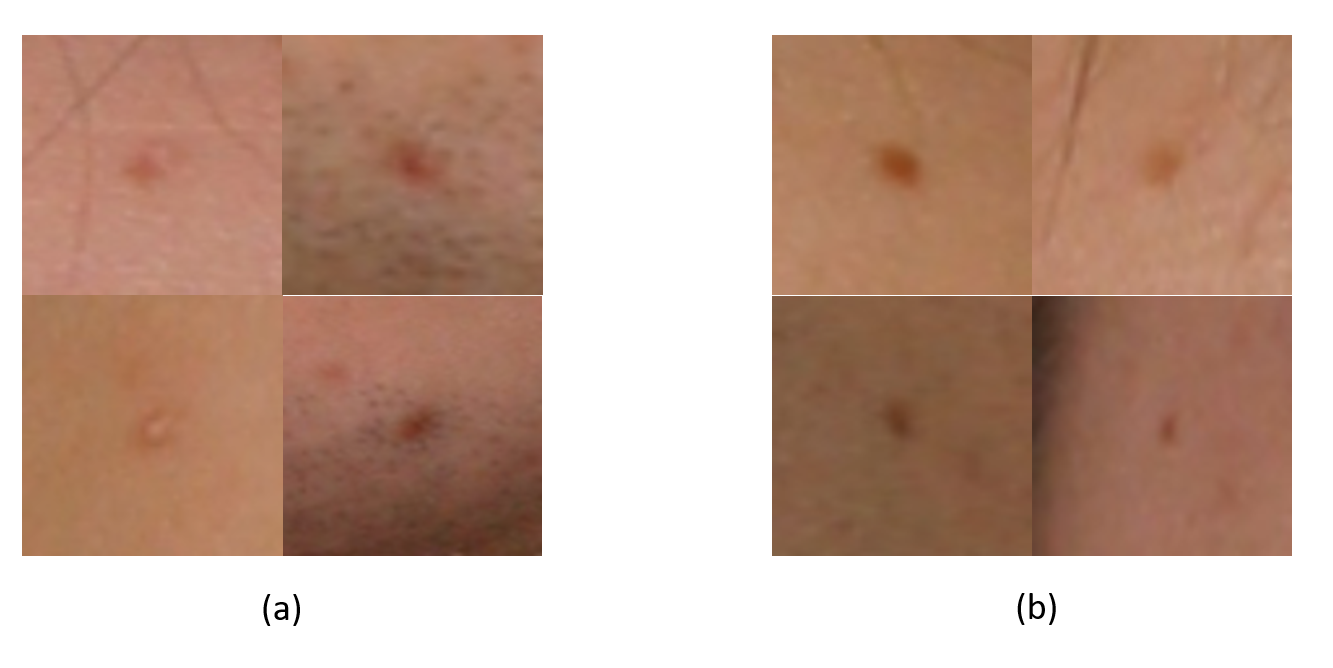
\includegraphics[width=\textwidth,height=\textheight,keepaspectratio]{per_vs_non}
	\caption{Examples of facials marks: (a) non-permanent, (b) permanent \label{fig:per_vs_non}}
\end{figure}
\FloatBarrier

This master thesis was started due to the need of combining the automatically calculated likelihood ratio value with the evidential value derived from the frequency of facial marks in certain regions of the face. The NFC is supporting this work by providing guidance and practical help.

\section{Related work}

A line of research relevant to this master thesis is the work by Vorder Bruegge et al. \cite{automatic_detector_2015} which proposed a fully automatic multiscale facial mark system. It detects facial marks which are stable across the the RGB-channels and different scales. These scales are called Gaussian pyramid and consist of low-pass filtered and subsampled images of the original image. This method to detect permanent marks are also used by Nisha Srinivas et al. \cite{twins} who tries to separate identical twins with an automatic multiscale facial mark detector. This method does not try to separate permanent and non-permanent facial mark rather tries to detect the more permanent marks.  

An other option considered when looking for facial marks are object detection and object classification.
The research on object detection and object classification is a wide and relevant field. Some of the things researchers have tried to detect and classify are faces \cite{facedetection_LBP}, pedestrians \cite{pedestrian_detection} and vehicles \cite{vehicle_hog}. These examples uses descriptive features based on histogram of oriented gradients (HOG) and local binary patterns (LBP). Face detectors also uses Haar-like features \cite{face_detection}. These three sets of features all describes the shape and structure of the searched object.

Taeg Sang Cho et al.\cite{reliable_mole} proposed a method using a Support Vector Machine (SVM) as a classifier to separate true and false mole candidates. They used a gist-descriptor as descriptive features. The gist-descriptor is designed to describe texture patterns over space. Read more about the gist-descriptor in the work of Antonio Torralba et al.\cite{gist_descriptor}. 

An other work using classifier are the work from Arfika Nurhudatiana et al. \cite{torso_RPPVSM}. They tried to detect and separate RPPVSM from non-RPPVSM on back torsos. They tried out three different classifiers which include a SVM, neural network and a binary decision tree. As input, the classifier was given the same set of features which included contrast, shape, size, texture, and color. Tim K. Lee et al.\cite{torso_mole} also used the same kind of features but does not use a trained classifier to separate true and false moles on back torsos. They use unsupervised algorithm to classify the mole candidates. 

When it comes to the detection of potential skin mark, there often involves some kind thresholding of a edge enhanced images. Using Laplacian of Gaussian (LoG) kernel as edge enhancement is popular method \cite{tattoos,face_matching}. After the edge enhancement of a image, the skin marks are highlighted and can then be segmented with different thresholding methods. 

\section{Motivation}

The work \cite{reliable_mole,torso_RPPVSM,torso_mole} all try to separate skin marks and they use a fixed set of features to do this. Arfika Nurhudatiana et al. compare different classifiers but there have been little work on comparing different set of features to separate permanent and non-permanent skin marks. This is why this thesis work will focus on comparing different features as input to a supervised classier. Since the facial marks have a circular shape and mostly vary in color it would bee wise to use colors maps as features. 

This master thesis will look at a recently used and interesting method to highlight the skin marks, instead of the common LoG kernel. The algorithm is called fast radial symmetry (FRS) \cite{twins,automatic_detector_2015} and it highlights radially symmetrical regions and suppresses regions that are asymmetrical. This is ideal when one is looking for circular objects which is perfect since facial marks are often circular. The FRS is expected to be more suitable for detecting skin marks compared to previous approaches, and is therefore investigated in this thesis.

The challenge with detecting skin marks, especially in the face, is that there are many other structures which can be mistaken as facial marks, e.g. nostrils, facial hair. Facial hair in the form of stubble can complicate the problems, as its appearance may be similar to a facial mark. The main challenge of this work is to find characteristic features for the permanent and non-permanent skin marks. They differ little in shape and structure but differ more in color. This master thesis will try to overcome these challenges. 


\section{Aim}

The aim of thie master thesis is to develop a method for creating a large data base with facial images and the location of facial marks. Such a database would provide better statistics for the evidential value in forensic facial image comparison examinations. The algorithm should detect facial marks automatically from a color image and then separate them into a permanent and non-permanent group.

\section{Problem specification}

From a single facial RGB-image en face, facial marks should be detected and classified as a permanent or non-permanent mark. This task can be divided into five smaller tasks. These task will be described more in detail in later chapters.

\textbf{\textit{Task 1: Pre-processing}}
The image can be illuminated unevenly and rotated which can cause difficulties when detection potential facial marks. Thus, the image has to be geometrically and photometrically normalized. 

\textbf{\textit{Task 2: Candidate detection}}
The actual detection of potential marks are done with the help of radial symmetry in the image. The algorithm will search for areas which contains edges that have a circular shape.   

\textbf{\textit{Task 3: Post-processing}}
Among the potential facial marks, there can be many false detections such as nostrils, facial hair, pupils et cetera. The false detection has to be eliminated and will be done with a hair removal method, blob identifier, size eliminator and face segmentation.

\textbf{\textit{Task 4: Classification}}
When the marks has been detected, they have to be sorted into the two classes, permanent and non-permanent. This is done by calculating different descriptive features. These features is used to train a supervised support vector machine. With the trained classifier, the facial mark can sorted. 

\textbf{\textit{Task 5: Feature selection}}
The major task in this master thesis is to compare and evaluate different descriptive features. This is done by choosing different sets of features for the classifier and evaluate the performance of the classifier for each set. 

\section{Scope}

In general, when working with image, the quality of the images are crucial for the results. Low resolution and badly illuminated images taken from different angles can cause analytical difficulties. Therefore, this thesis assumes images which are high resolute, well illuminated, taken en face and in RGB-colours. 

Also, this master thesis will focus on a comparison between different sets of features for the classifier instead of examining different ways of detecting facial marks. This is due to the little work done regarding feature selection. 

The classifier will only be a binary classifier because no non-facial marks has been collected as labelled data during the thesis work due to lack of resources.   

\section{Thesis outline}

This chapter describes the aim and problem specification of this master thesis. In Chapter \ref{cha:theory}, gives an insight in theory behind the methods used in the algorithm. Chapter \ref{cha:method} describes the pipeline of the algorithm and the implementation of the theory used in it. The results from the algorithm can be studied in Chapter \ref{cha:result} and an discussion about the result and methods used is found in Chapter \ref{cha:Discussion}. Finally, Chapter \ref{cha:conclusion} consist of a conclusion of the master thesis and ideas for future work within the same scope. 